\chapter{Proposed Study Design}
Given the scope from chapter 2 and the parameters from chapter 3, this chapter proposes a study design. The study aims to produce data to answer the main research question from chapter 1:
\begin{itemize}
	\item[MRQ] Does the visual perspective on a virtual guidance visualisation have an influence on motor learning in MR environments.
\end{itemize}

\section{Setup}
For the study, a movement training system will be implemented. This movement training system will include a virtual reality HMD and motion-tracking technology. The student will be tracked with this motion capturing technology and with the resulting information, the student's avatar will be rendered as a high realism degree avatar. Likewise, the teacher avatar will be rendered, but not on the base of live motion tracking data. A professional Tai Chi trainer will be invited and a Tai Chi form will be recorded. This form will be split into 4 sub-forms. Furthermore, the teacher avatar will be scaled to the size of the student's avatar. To overcome the mirror issue, the student is allowed to move freely around the teachers' avatar. During the students' performance, the movement will be recorded and analysed in the aftermath with the discussed performance measure. 

\section{Procedure}
The study is conducted in a within-subject design with counterbalancing, which results in 32 participants, compare table~\ref{tbl:studySetting}. The student starts with the first visual perspective. The teacher appears and performs the movement, while the student is watching the performance. After the first demonstration, the student can train the motion simultaneously until the student is feeling confident, but caps after an amount of time which a pilot study has to reveal. After one of these cases, the final movement will be recorded, the student gets a short recovery rest. Then the next visual perspective starts. This process continues throughout all four conditions. Subsequent to the actual study, the post questionnaires will be answered. This questionnaire will contain questions about, perceived precision, ease to understand an preferred method.

\begin{table}
	\centering
	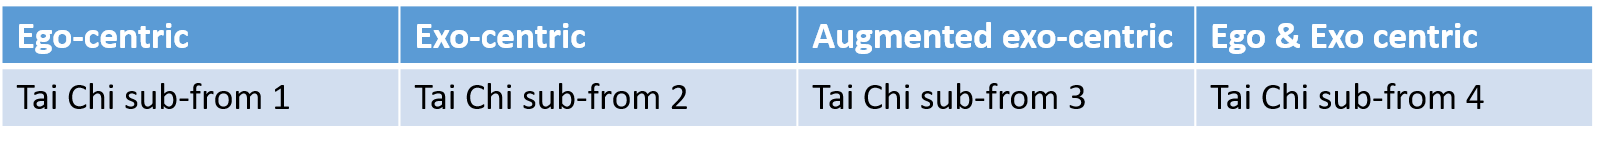
\includegraphics[width=1.0\textwidth]{img/studySetting.png}
	\caption{Study conduction schema.}
	\label{tbl:studySetting}
\end{table}

\section{Outlook}
The next step is to implement the study setup, but still, there are some parameters to refine on. This takes place in the master's project. In this part, the technology and algorithms will be in the main focus. For technology, VR HMDs will be compared and a decision will be made. Similar to motion tracking technologies. After this, algorithms for comparing two movements will be evaluated. When decisions are made, the implementation of the system will start. Eventually, a pilot testing session will take place followed by further refinements.
The milestones for the master's project are:
\begin{itemize}
	\item Hardware requirements: 17.1.2020
	\item Software Requirements: 24.1.2020
	\item Implementation Start: 27.1.2020
	\item Pilot Study: 2.3.2020
	\item Refinements Implementation: 13.3.2020
	\item Master’s Project Presentation and Report: 23.3.2020
\end{itemize}
The thesis will follow in the summer semester 2020. The results are planned to be published at a conference in 2020, compare figure~\ref{fig:outlook}.\\
For the master's thesis, a study will be conducted. The study will generate data to answer the research question. This data will be analysed in detail and eventually be used to answer the research question.

\begin{figure}
	\centering
	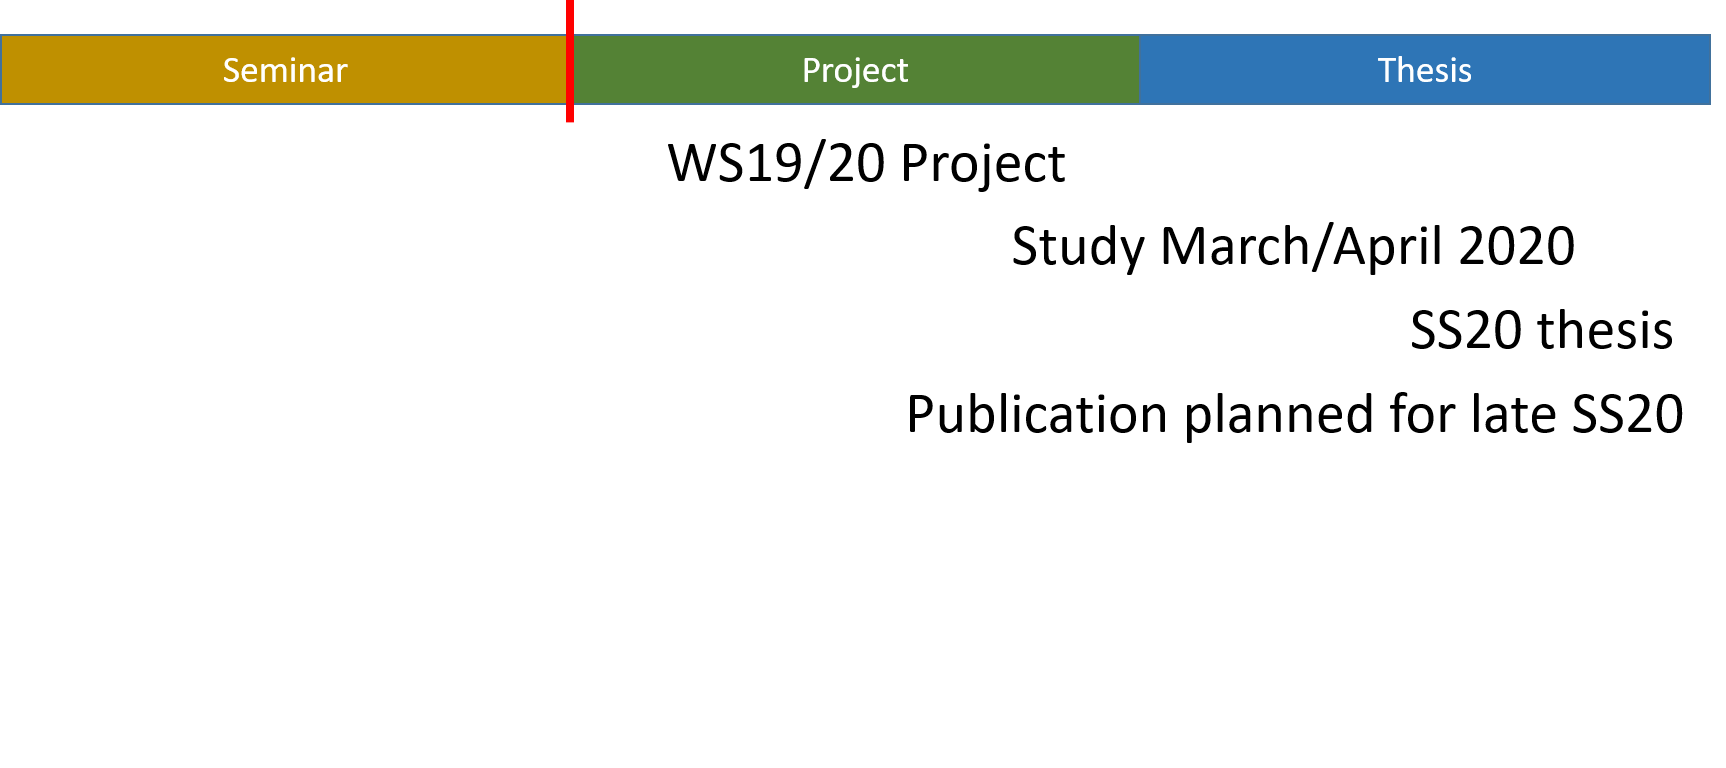
\includegraphics[width=1.0\textwidth]{img/outlook.png}
	\caption{Timetable for the master's thesis.}
	\label{fig:outlook}
\end{figure}

\begin{comment}
\section{Variables}
\subsection{Independent Variables}
\begin{itemize}
\item ego-centric
\item exo-centric
\item combined
\begin{itemize}
\item \textcolor{red}{variation of combined:} sequetial - parallel
\end{itemize}
\end{itemize}
further variations that could be interesting:
\begin{itemize}
\item body parts
\item sitting/standing
\item visual representation
\item degree of realism of avatar
\item guidance techniques: stopping at keyframes vs. fluent instructions
\item audio queues
\item feedback
\item fixed position of teacher and avatar, vs walking around
\end{itemize}
\subsection{Dependent variables}
Score. Combination of objective and subjective measurements.
\begin{itemize}
\item precision
\item subjective opinion of participant
\item stress level (EKG, HRV)
\item cognitive load
\item retention
\item reaction time
\end{itemize}
\section{Task}
\begin{itemize}
\item Tai Chi form, split in subtasks
\item Dance moves from single dance
\end{itemize}
variations:
\begin{itemize}
\item difficulty
\item complexity
\item abstract vs. real world
\item operate a control panel
\item escape the room
\item game    
\end{itemize}

\section{Hypothesis}
%hier wird ein mögliches studiendesign vorgestellt

\subsection{Aim of the Study}
The aim of the study is to investigate the influence of egocentric and exocentric perspectives on a virtual avatar during motor learning tasks.

\subsection{process}
There are two groups: one learn only with the egocentric perspective, the other one with the exocentric perspective on the virtual avatar.\\
To derive conclusions on body regions, every participant learns movements for three different body parts. The body parts are:
\begin{itemize}
\item \UB (UB)
\item \LB (LB)
\item \FB (FB)
\end{itemize}
To derive conclusion on movement types, two different movements per body part is learned. The two movement types are:
\begin{itemize}
\item mirrored movements
\item independent movements
\end{itemize}

\begin{center}
\begin{tabular}{ | c | c | c | c | }
\hline
& UB & LB & FB \\ \hline 
Ego & \parbox{4cm}{1 mirrored and 1 asynchronous movement} & \parbox{4cm}{1 mirrored and 1 independent movement} & \parbox{4cm}{1 mirrored and 1 independent movement} \\ \hline 
Exo & \parbox{4cm}{1 mirrored and 1 independent movement} & \parbox{4cm}{1 mirrored and 1 independent movement} & \parbox{4cm}{1 mirrored and 1 independent movement} \\ \hline
Ego/Exo & \parbox{4cm}{1 mirrored and 1 independent movement} & \parbox{4cm}{1 mirrored and 1 independent movement} & \parbox{4cm}{1 mirrored and 1 independent movement} \\
\hline
\end{tabular}
\label{table:studyDesign}
\end{center}

\subsection{Independent variables}
\begin{itemize}
\item perspective on the avatar (Ego/Exo centric)
\item body parts (\UB, \LB, \FB)
\item movement types (mirrored/independent movements)
\end{itemize}

\subsection{measures}
TBA
\end{comment}